\chapter{Evaluation}\label{sec:evaluation}

\begin{itemize}
    \item Top k: predicted class is within the top k predictions
    \item calculation for top k: 
    \[\frac{\binom{NUM\_CLASSES - 1}{k - 1}}{\binom{NUM\_CLASSES}{k}} = \frac{k}{NUM\_CLASSES}\]
    \item for the floor with most files: NUM\_CLASSES = 4795
    \item Probabilities to pick one random \ac{bssid}, and it is the right one in top 3, 5 or 10, see \cref{fig:random_accuracies_4795_classes}
    \item Accuracy of the model's prediction with a batch\_size of 32, see \cref{fig:window_size3},\cref{fig:window_size5},\cref{fig:window_size10} and \cref{fig:window_size20}
    \item Accuracy of the model's prediction with a batch\_size of 16, see \cref{fig:window_size10_batch16}
    \item Accuracy of the model's prediction with a batch\_size of 64, see \cref{fig:window_size10_batch64}
\end{itemize}

\begin{figure}[h!]
    \centering
    \includegraphics*[scale=0.8]{images/random_accuracies_4795_classes.png}
    \caption{Probabilities that the predicted class falls within the top k randomly selected classes.}
    \label{fig:random_accuracies_4795_classes}
\end{figure}

\begin{figure}[h!]
    \centering
    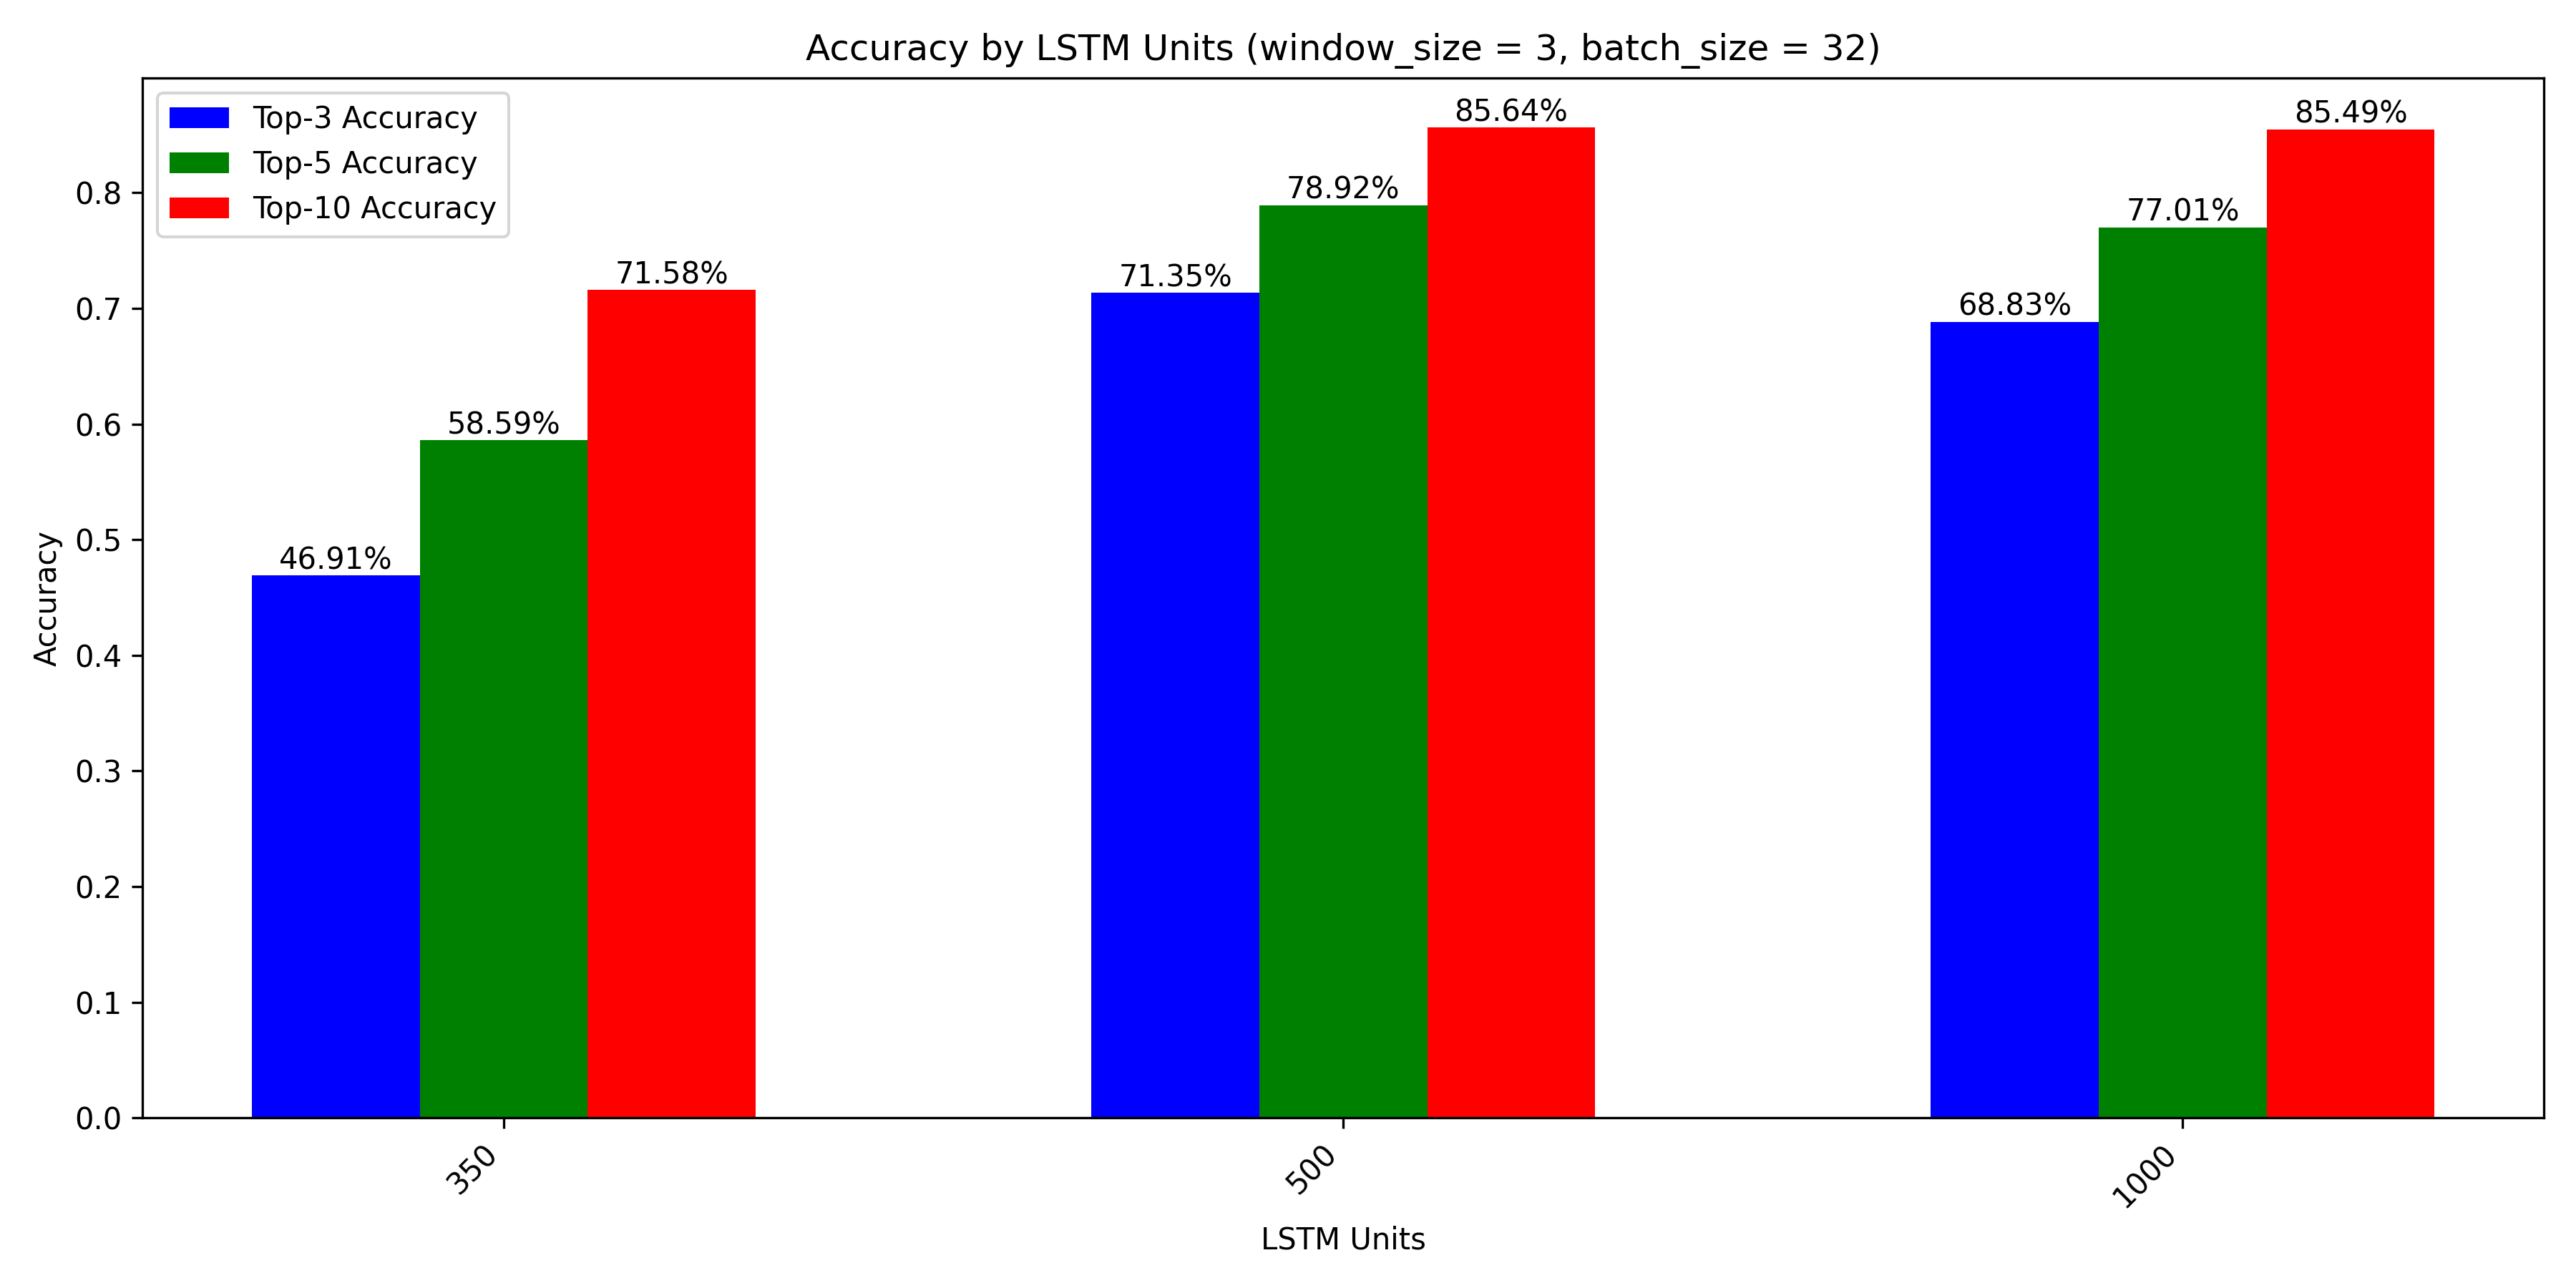
\includegraphics[scale=0.4]{images/accuracy_by_lstm_units_window_3_batch_32.png}
    \caption{Accuracy of the model with window size of 3, batch size of 32 and 100, 500 and 1000 units in the LSTM layer.}
    \label{fig:window_size3}
\end{figure}

\begin{figure}[h!]
    \centering
    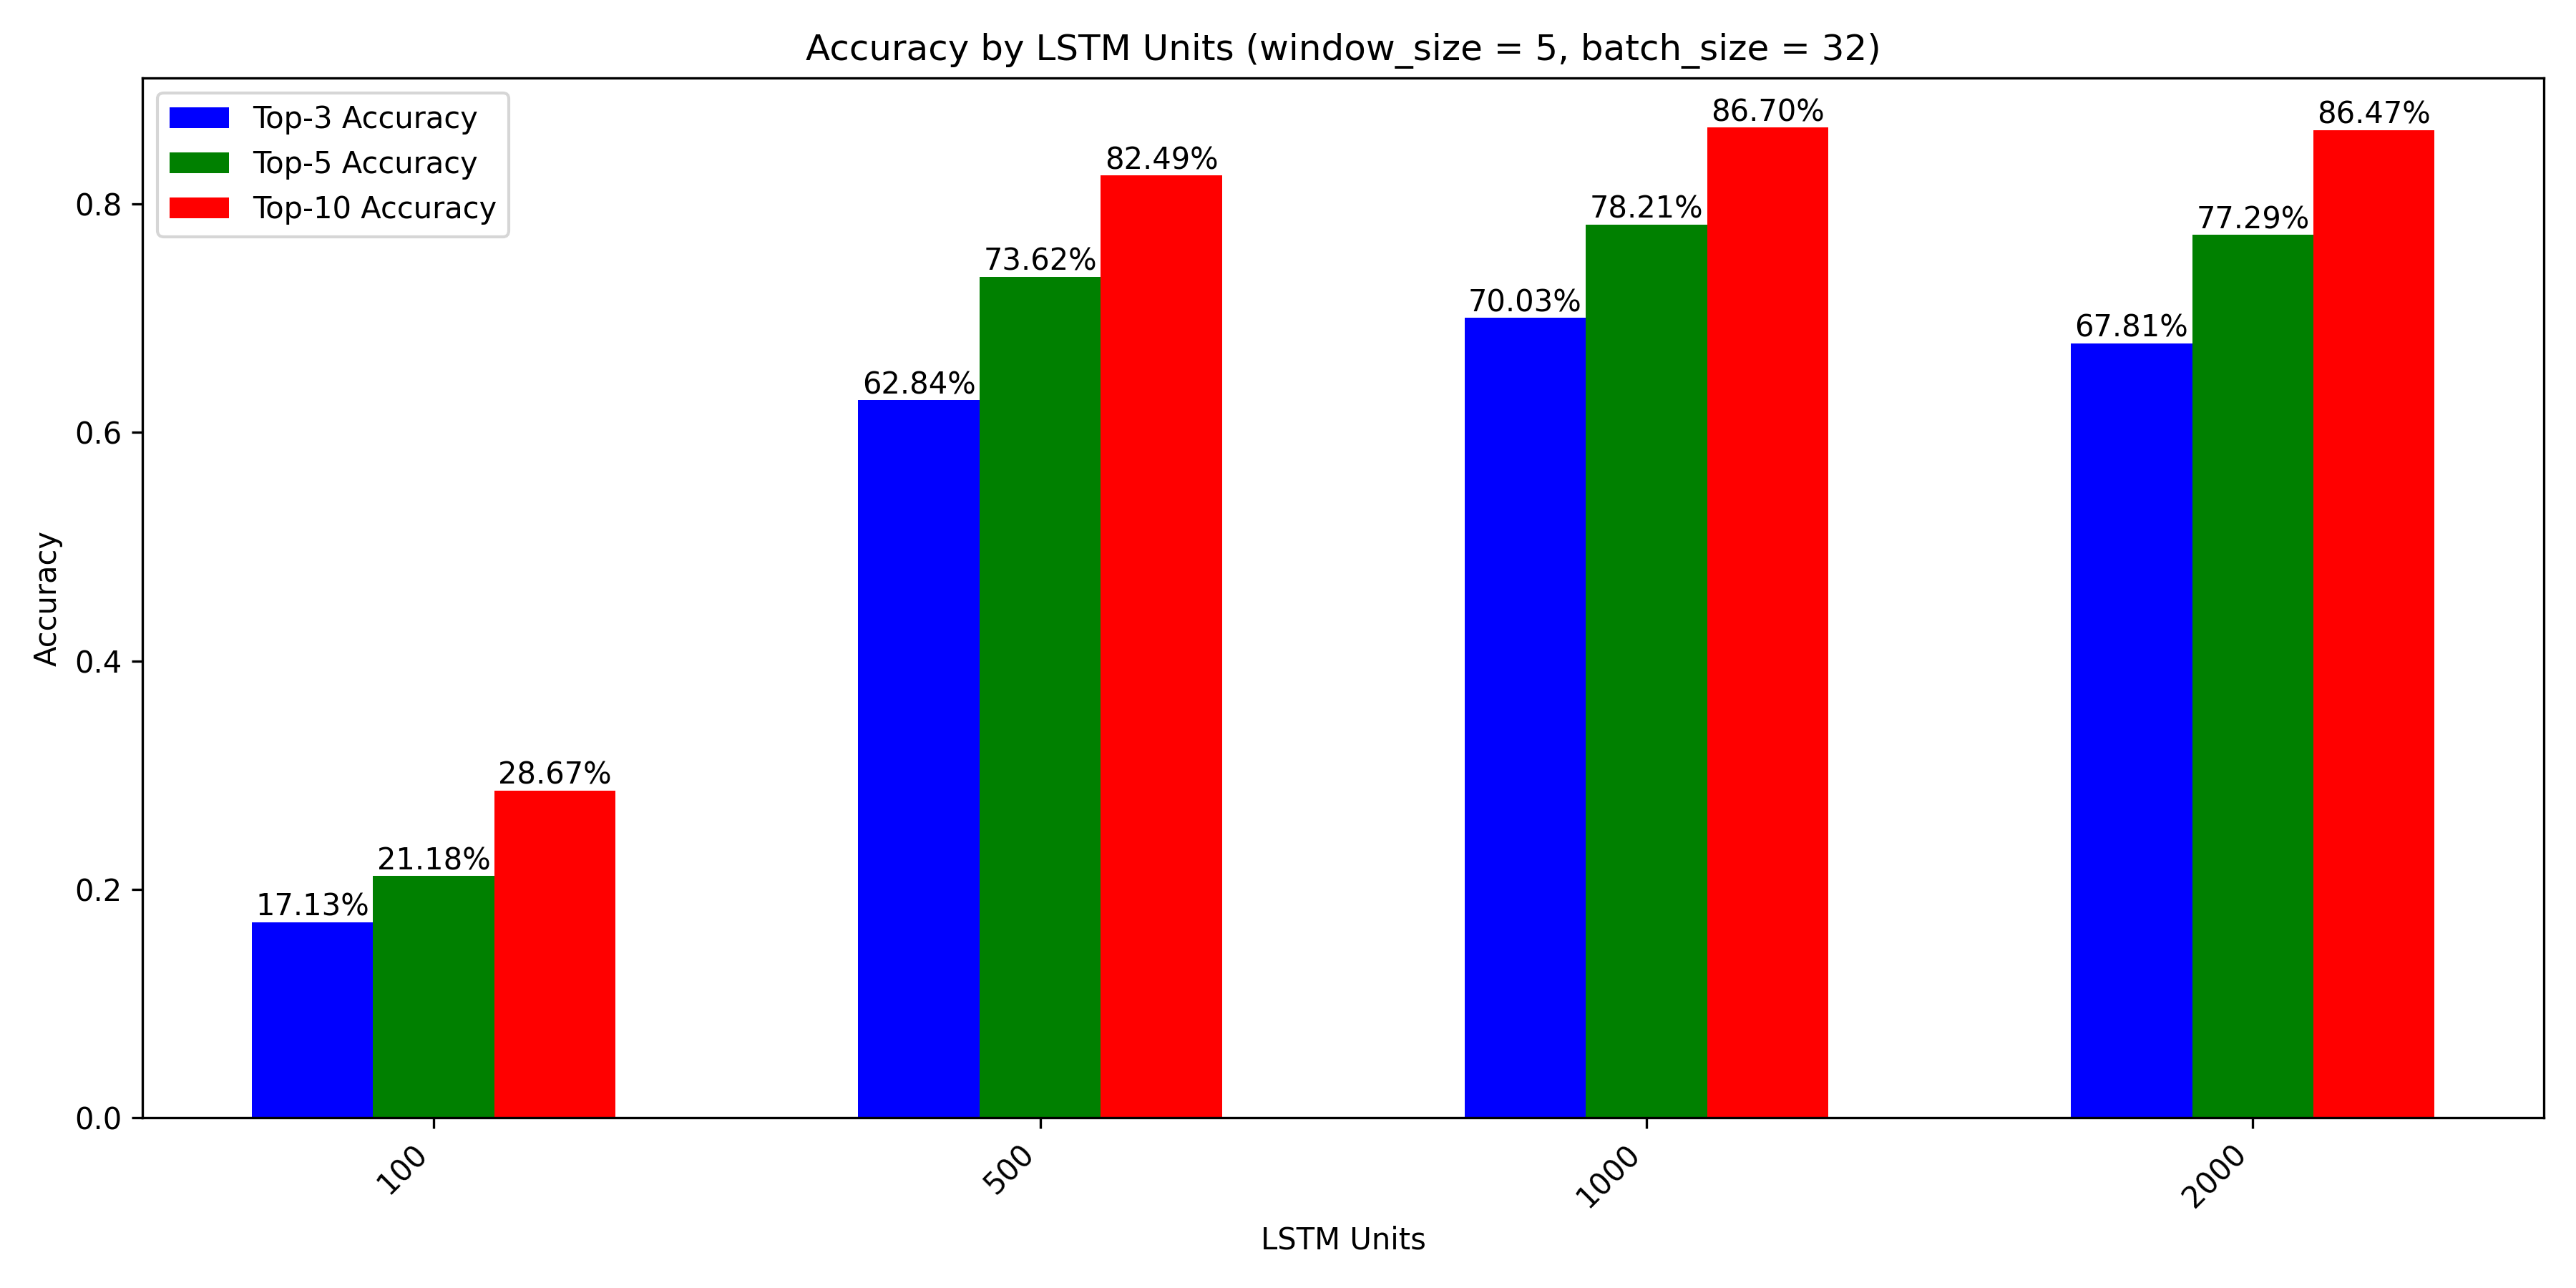
\includegraphics[scale=0.4]{images/accuracy_by_lstm_units_window_5_batch_32.png}
    \caption{Accuracy of the model with window size of 5, batch size of 32 and 100, 500 and 1000 units in the LSTM layer.}
    \label{fig:window_size5}
\end{figure}

\begin{figure}[h!]
    \centering
    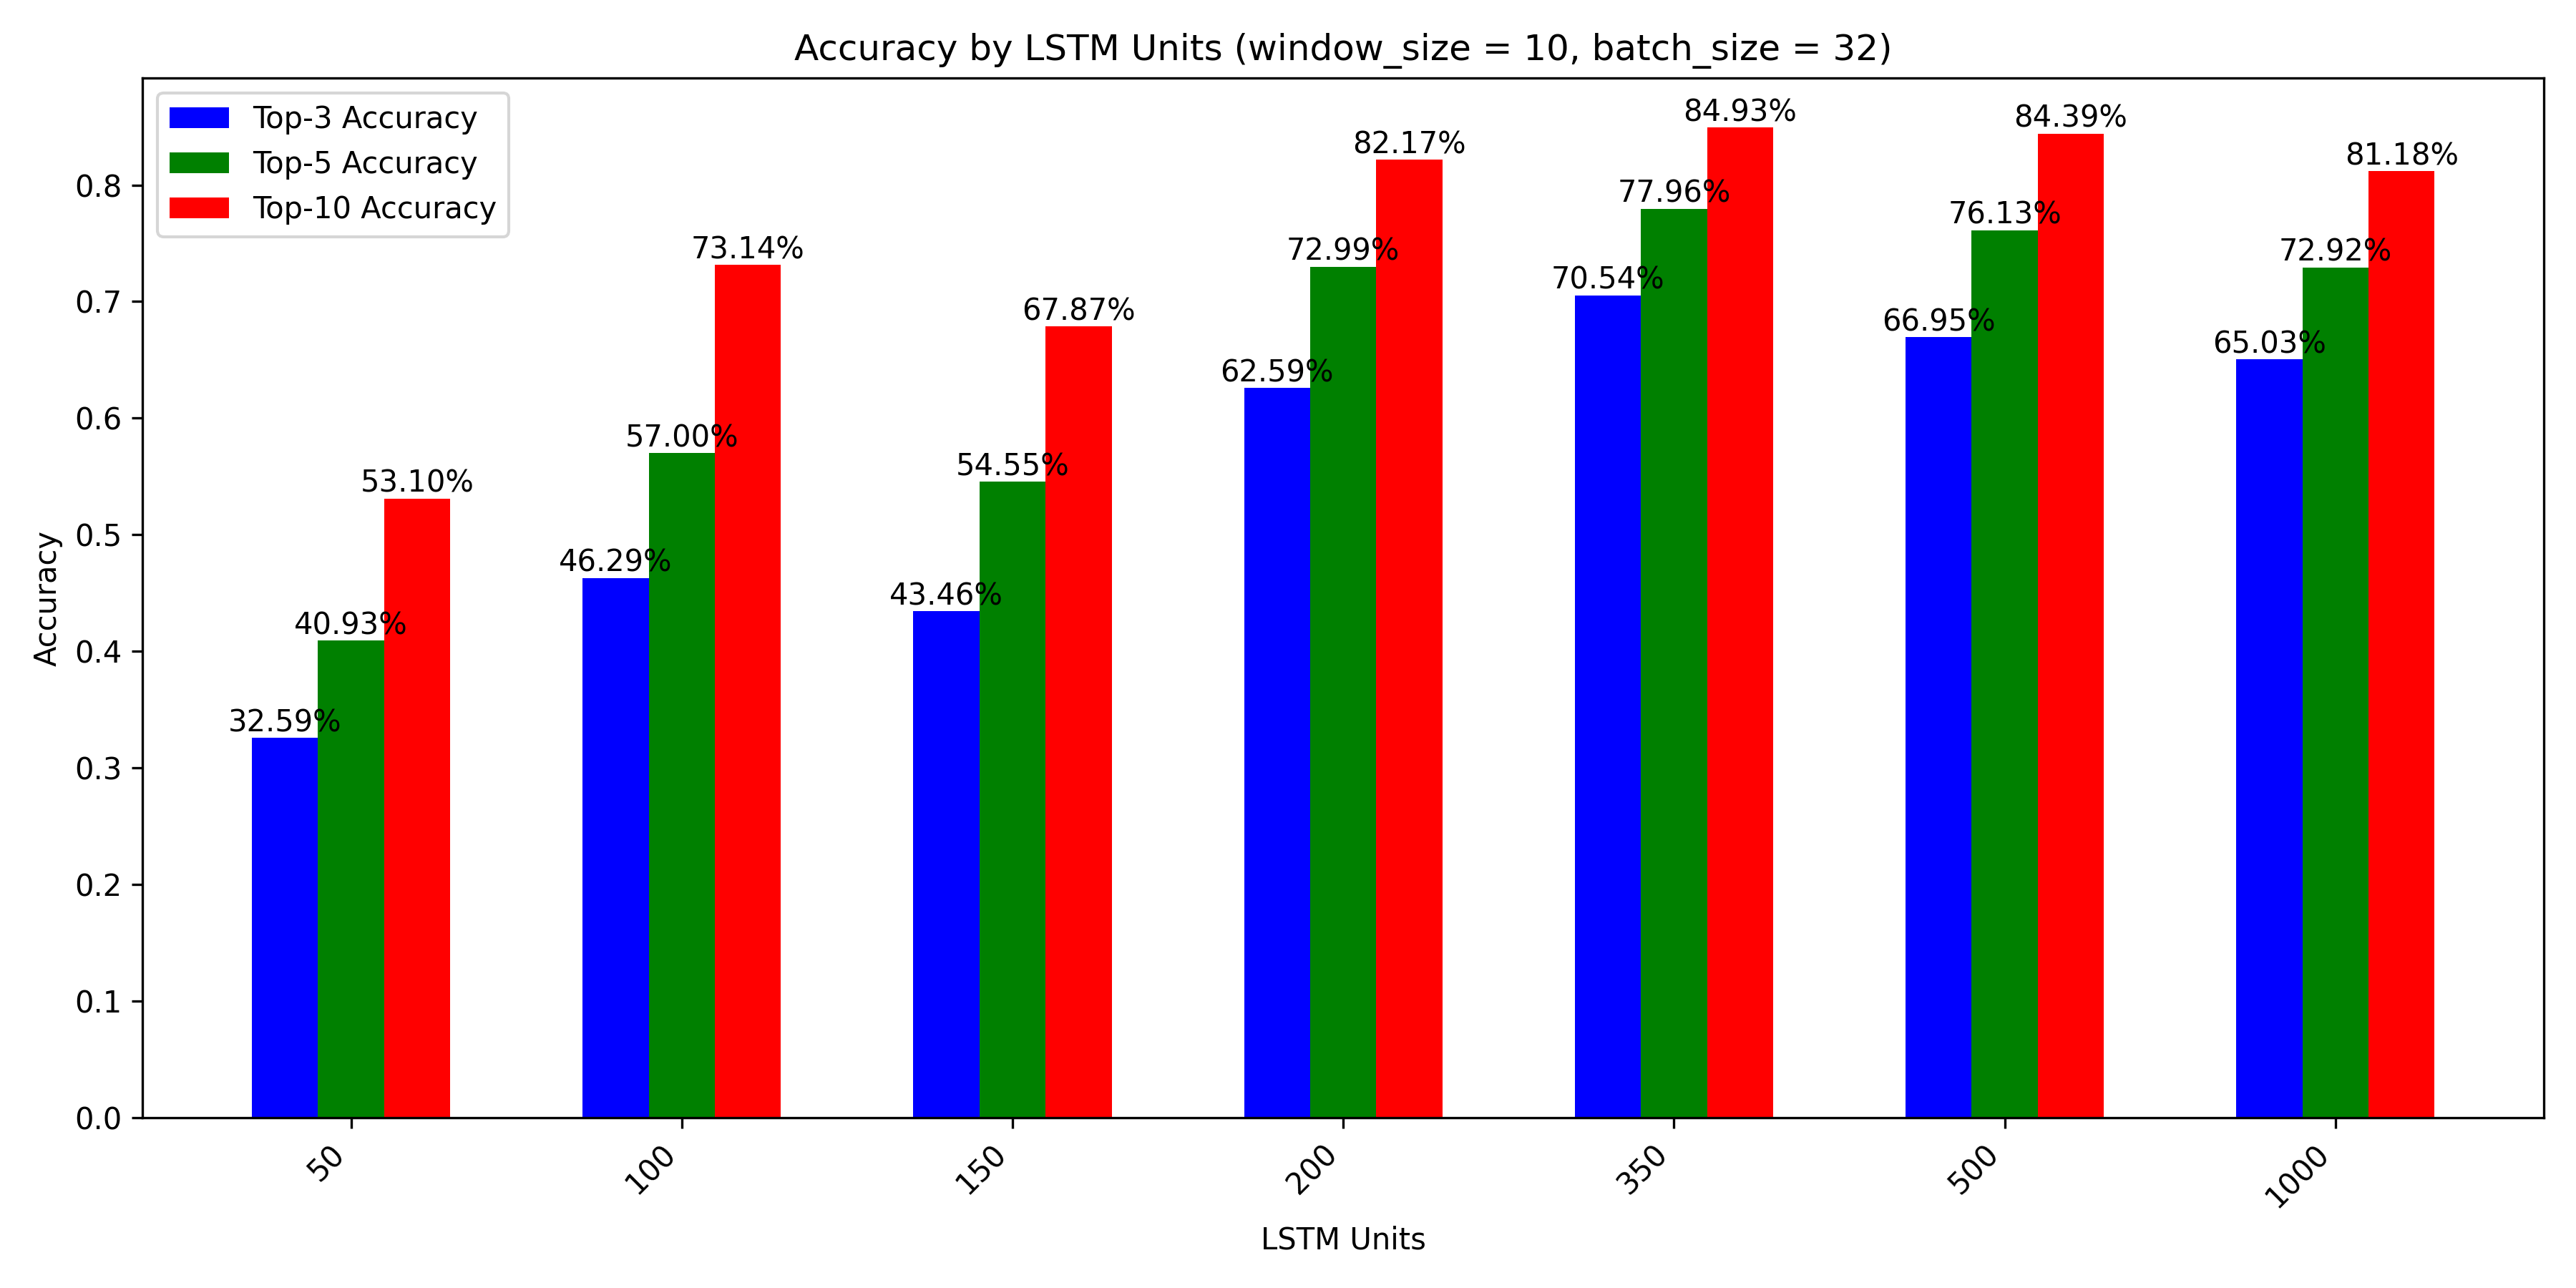
\includegraphics[scale=0.4]{images/accuracy_by_lstm_units_window_10_batch_32.png}
    \caption{Accuracy of the model with window size of 10, batch size of 32 and 100, 500 and 1000 units in the LSTM layer.}
    \label{fig:window_size10}
\end{figure}


\begin{figure}[h!]
    \centering
    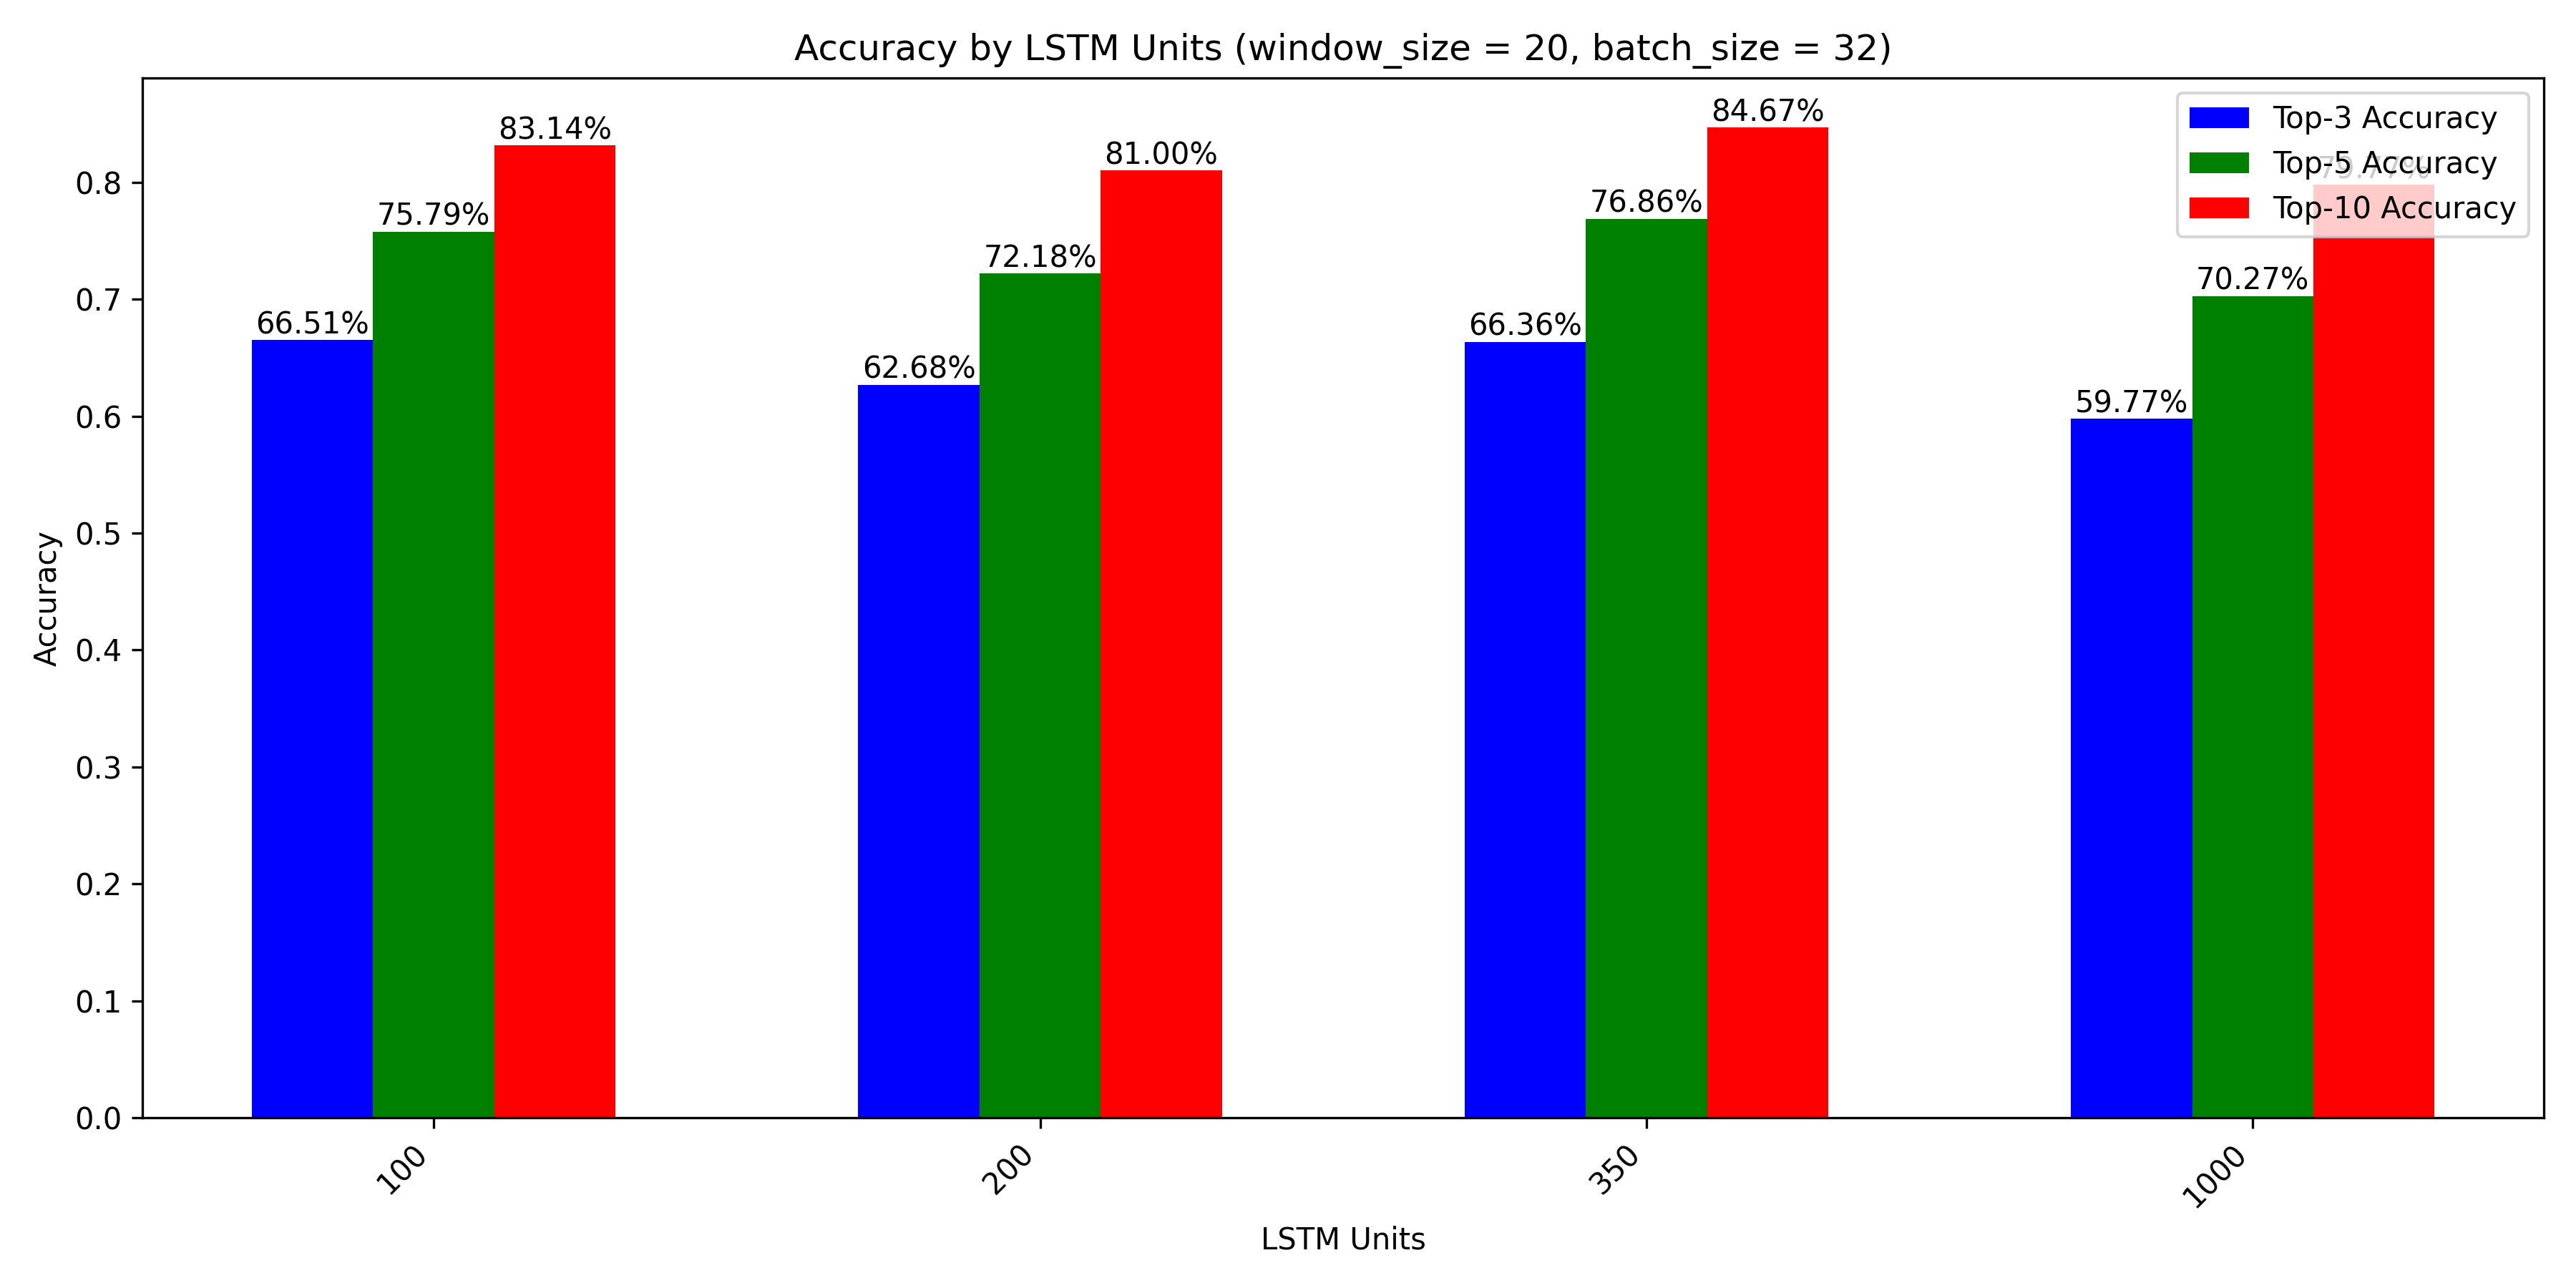
\includegraphics[scale=0.4]{images/accuracy_by_lstm_units_window_20_batch_32.png}
    \caption{Accuracy of the model with window size of 20, batch size of 32 and 100, 500 and 1000 units in the LSTM layer.}
    \label{fig:window_size20}
\end{figure}

\begin{figure}[h!]
    \centering
    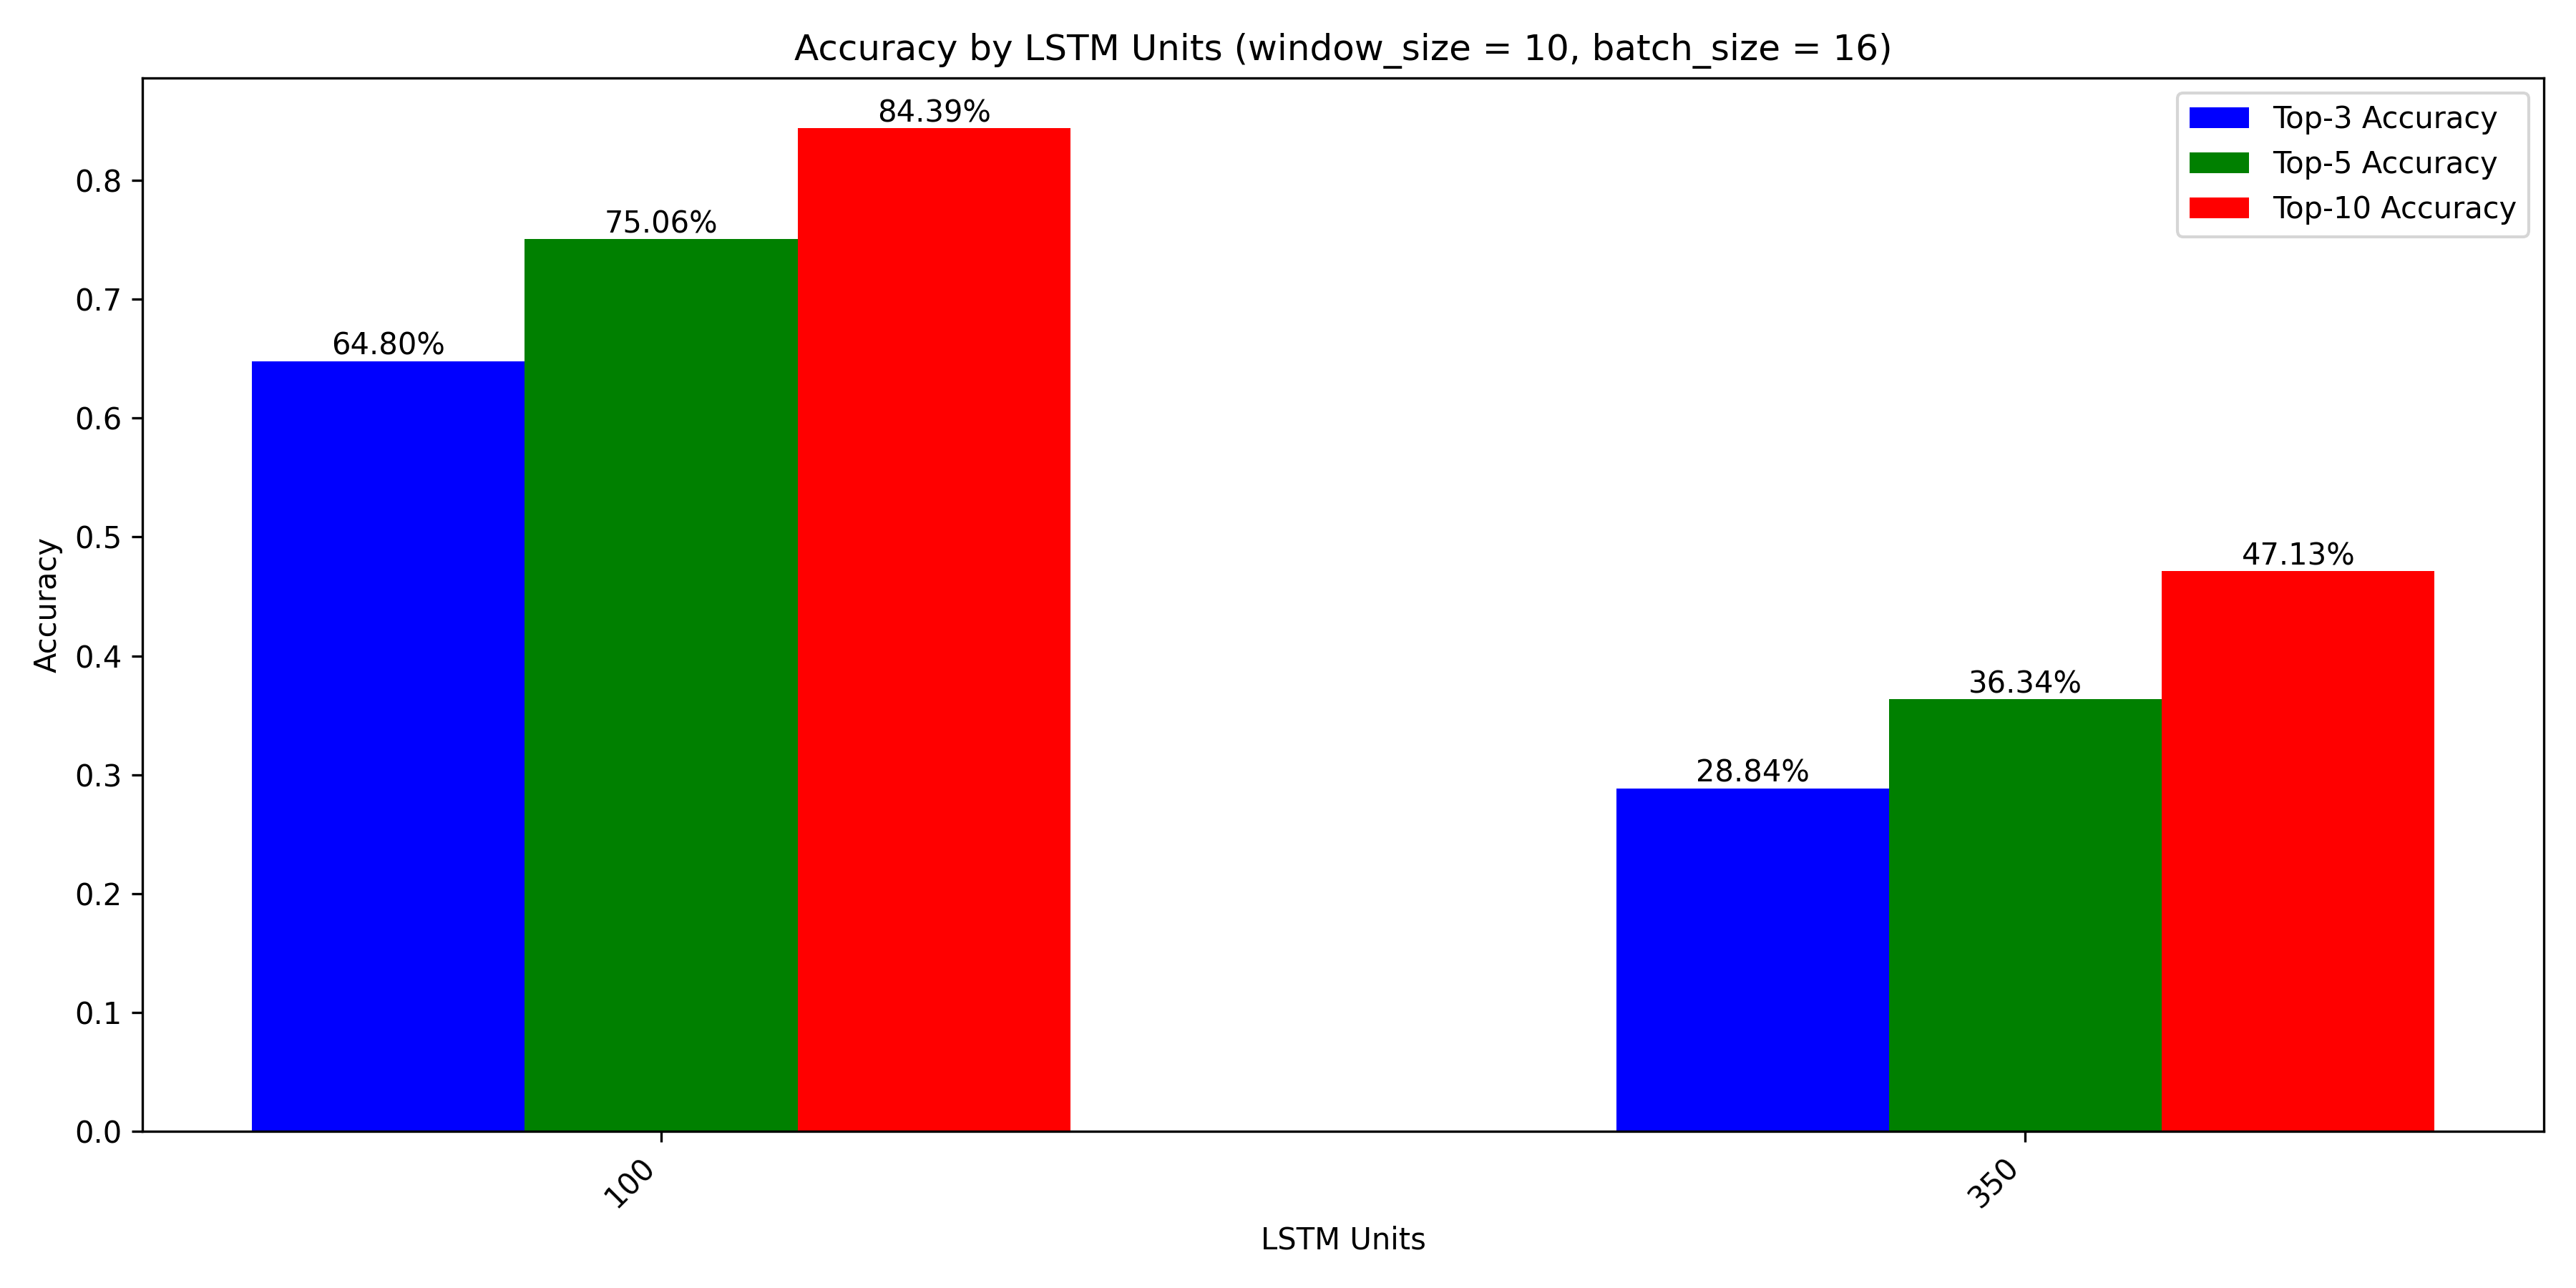
\includegraphics[scale=0.4]{images/accuracy_by_lstm_units_window_10_batch_16.png}
    \caption{Accuracy of the model with window size of 10, batch size of 16 and 100, 500 and 1000 units in the LSTM layer.}
    \label{fig:window_size10_batch16}
\end{figure}

\begin{figure}[h!]
    \centering
    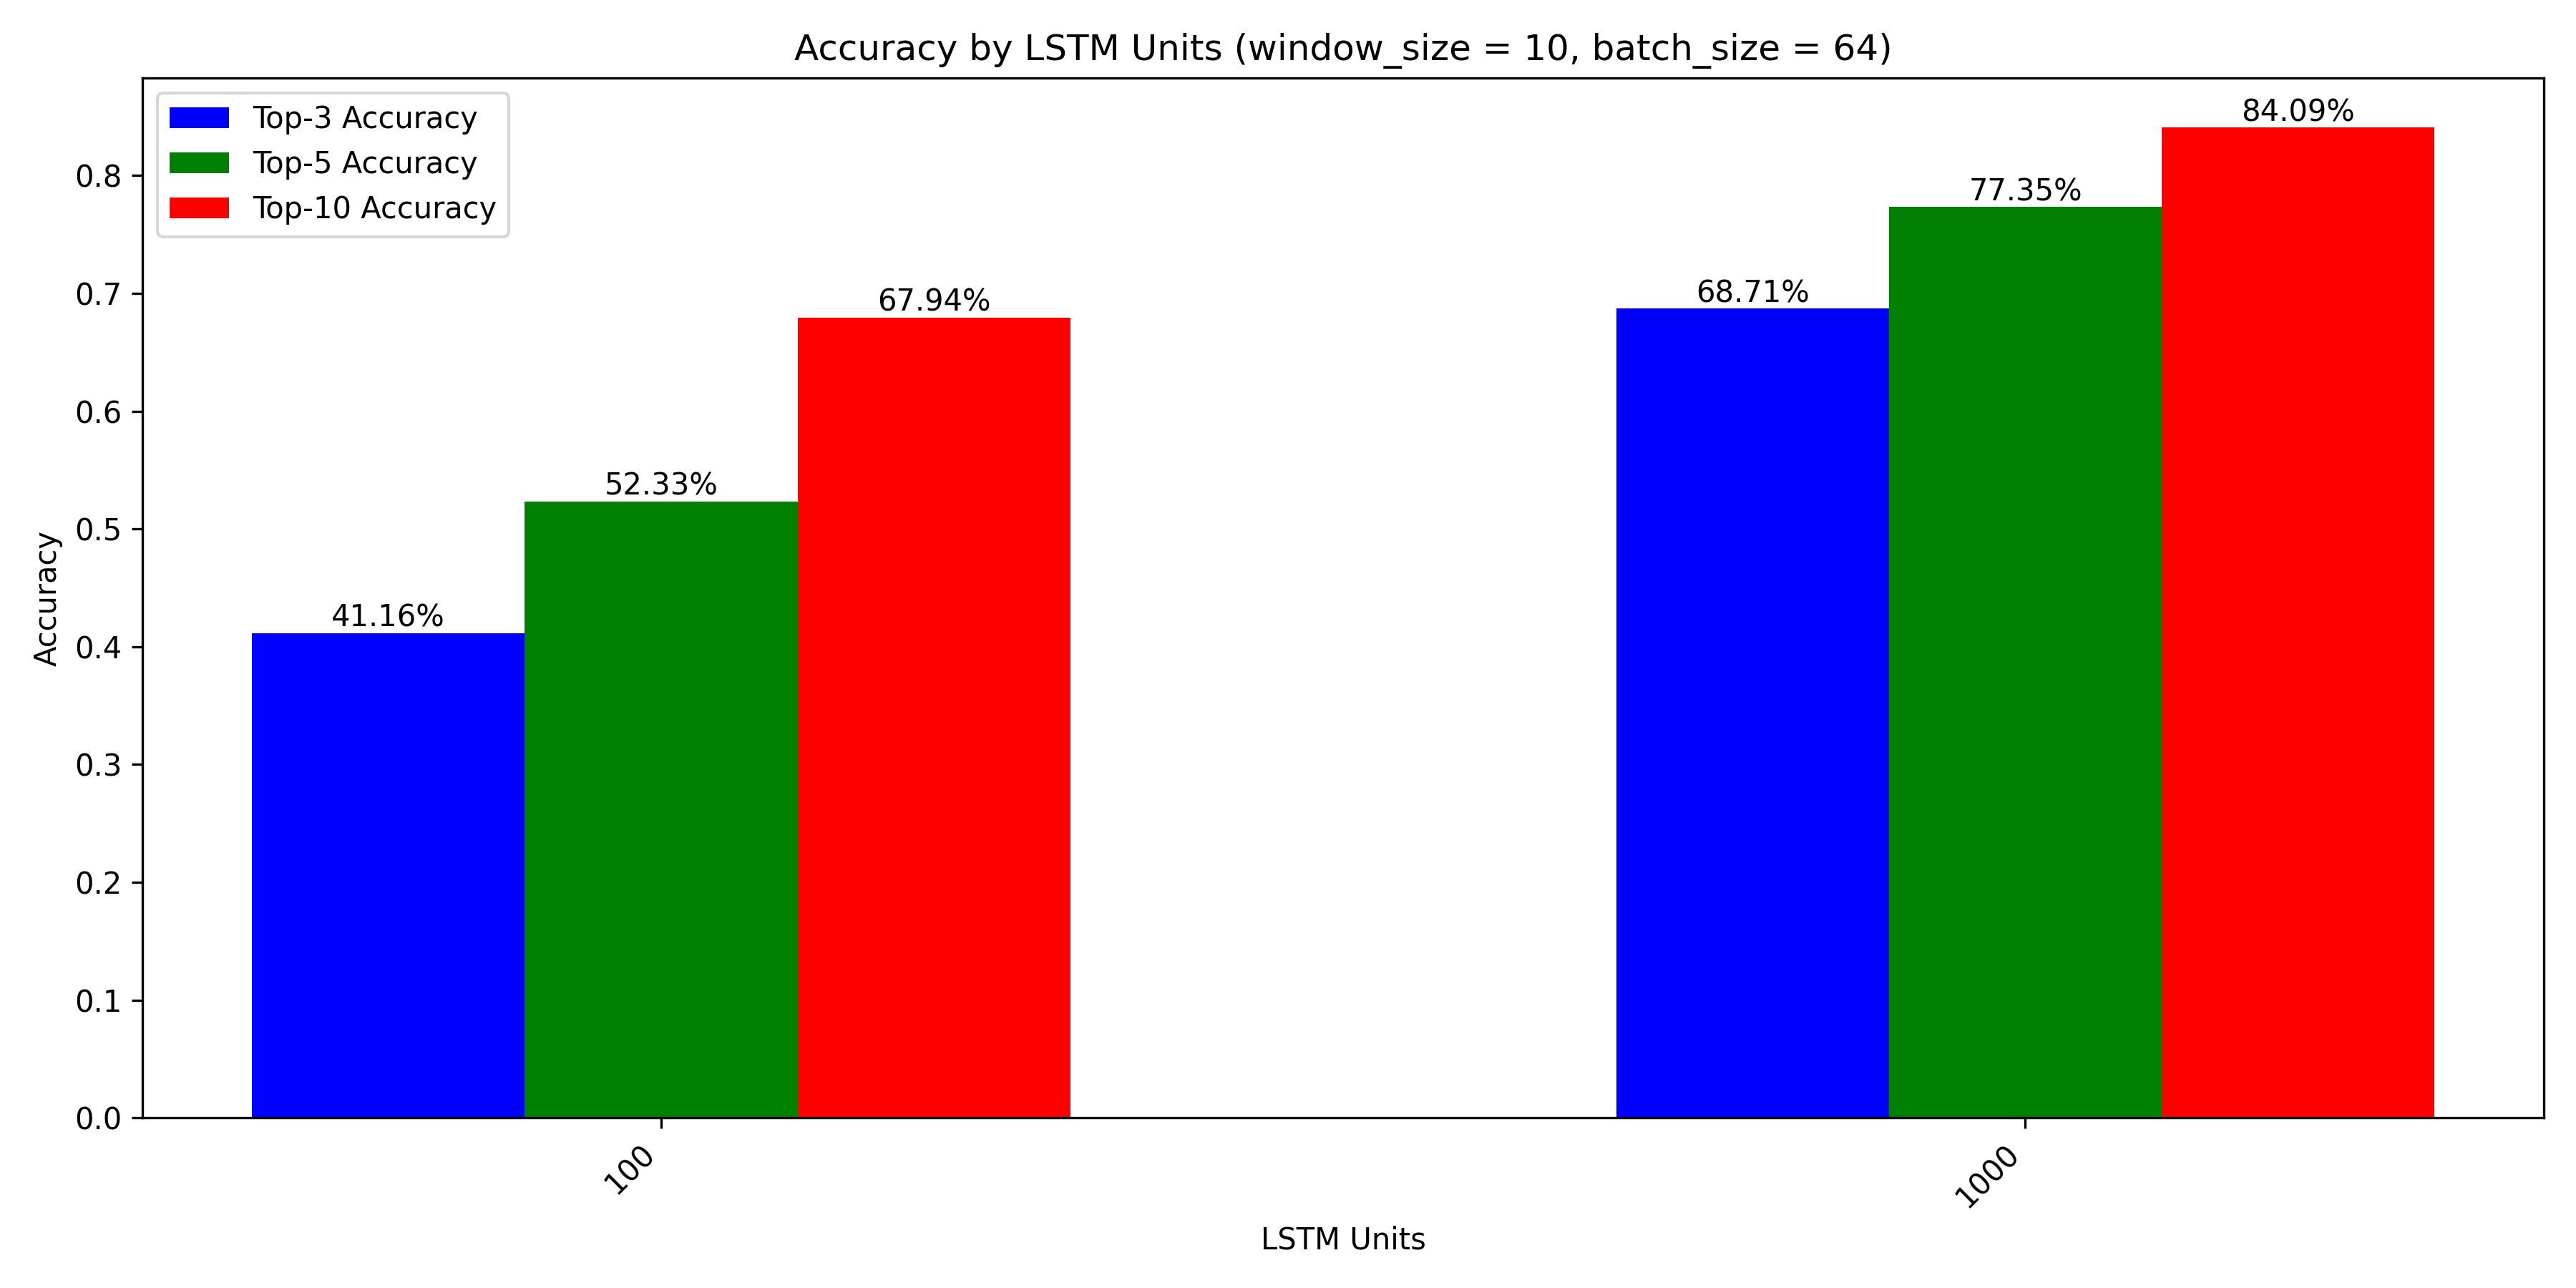
\includegraphics[scale=0.4]{images/accuracy_by_lstm_units_window_10_batch_64.png}
    \caption{Accuracy of the model with window size of 10, batch size of 64 and 100, 500 and 1000 units in the LSTM layer.}
    \label{fig:window_size10_batch64}
\end{figure}

\begin{itemize}
    \item Comparison with random selection of classes: lstm always better than random selection
    \item describing the plots
    \item best performance: 71\%, see \cref{fig:top3_best_models}
    \item Reasons:
    \subitem data contains too many classes, with fewer classes to predict the model could have performed better
    \subitem discussion could have missed a better model
    \subitem model very simple, could be improved by using other layers in between LSTM and Dense layers
\end{itemize}

\begin{figure}[h!]
    \centering
    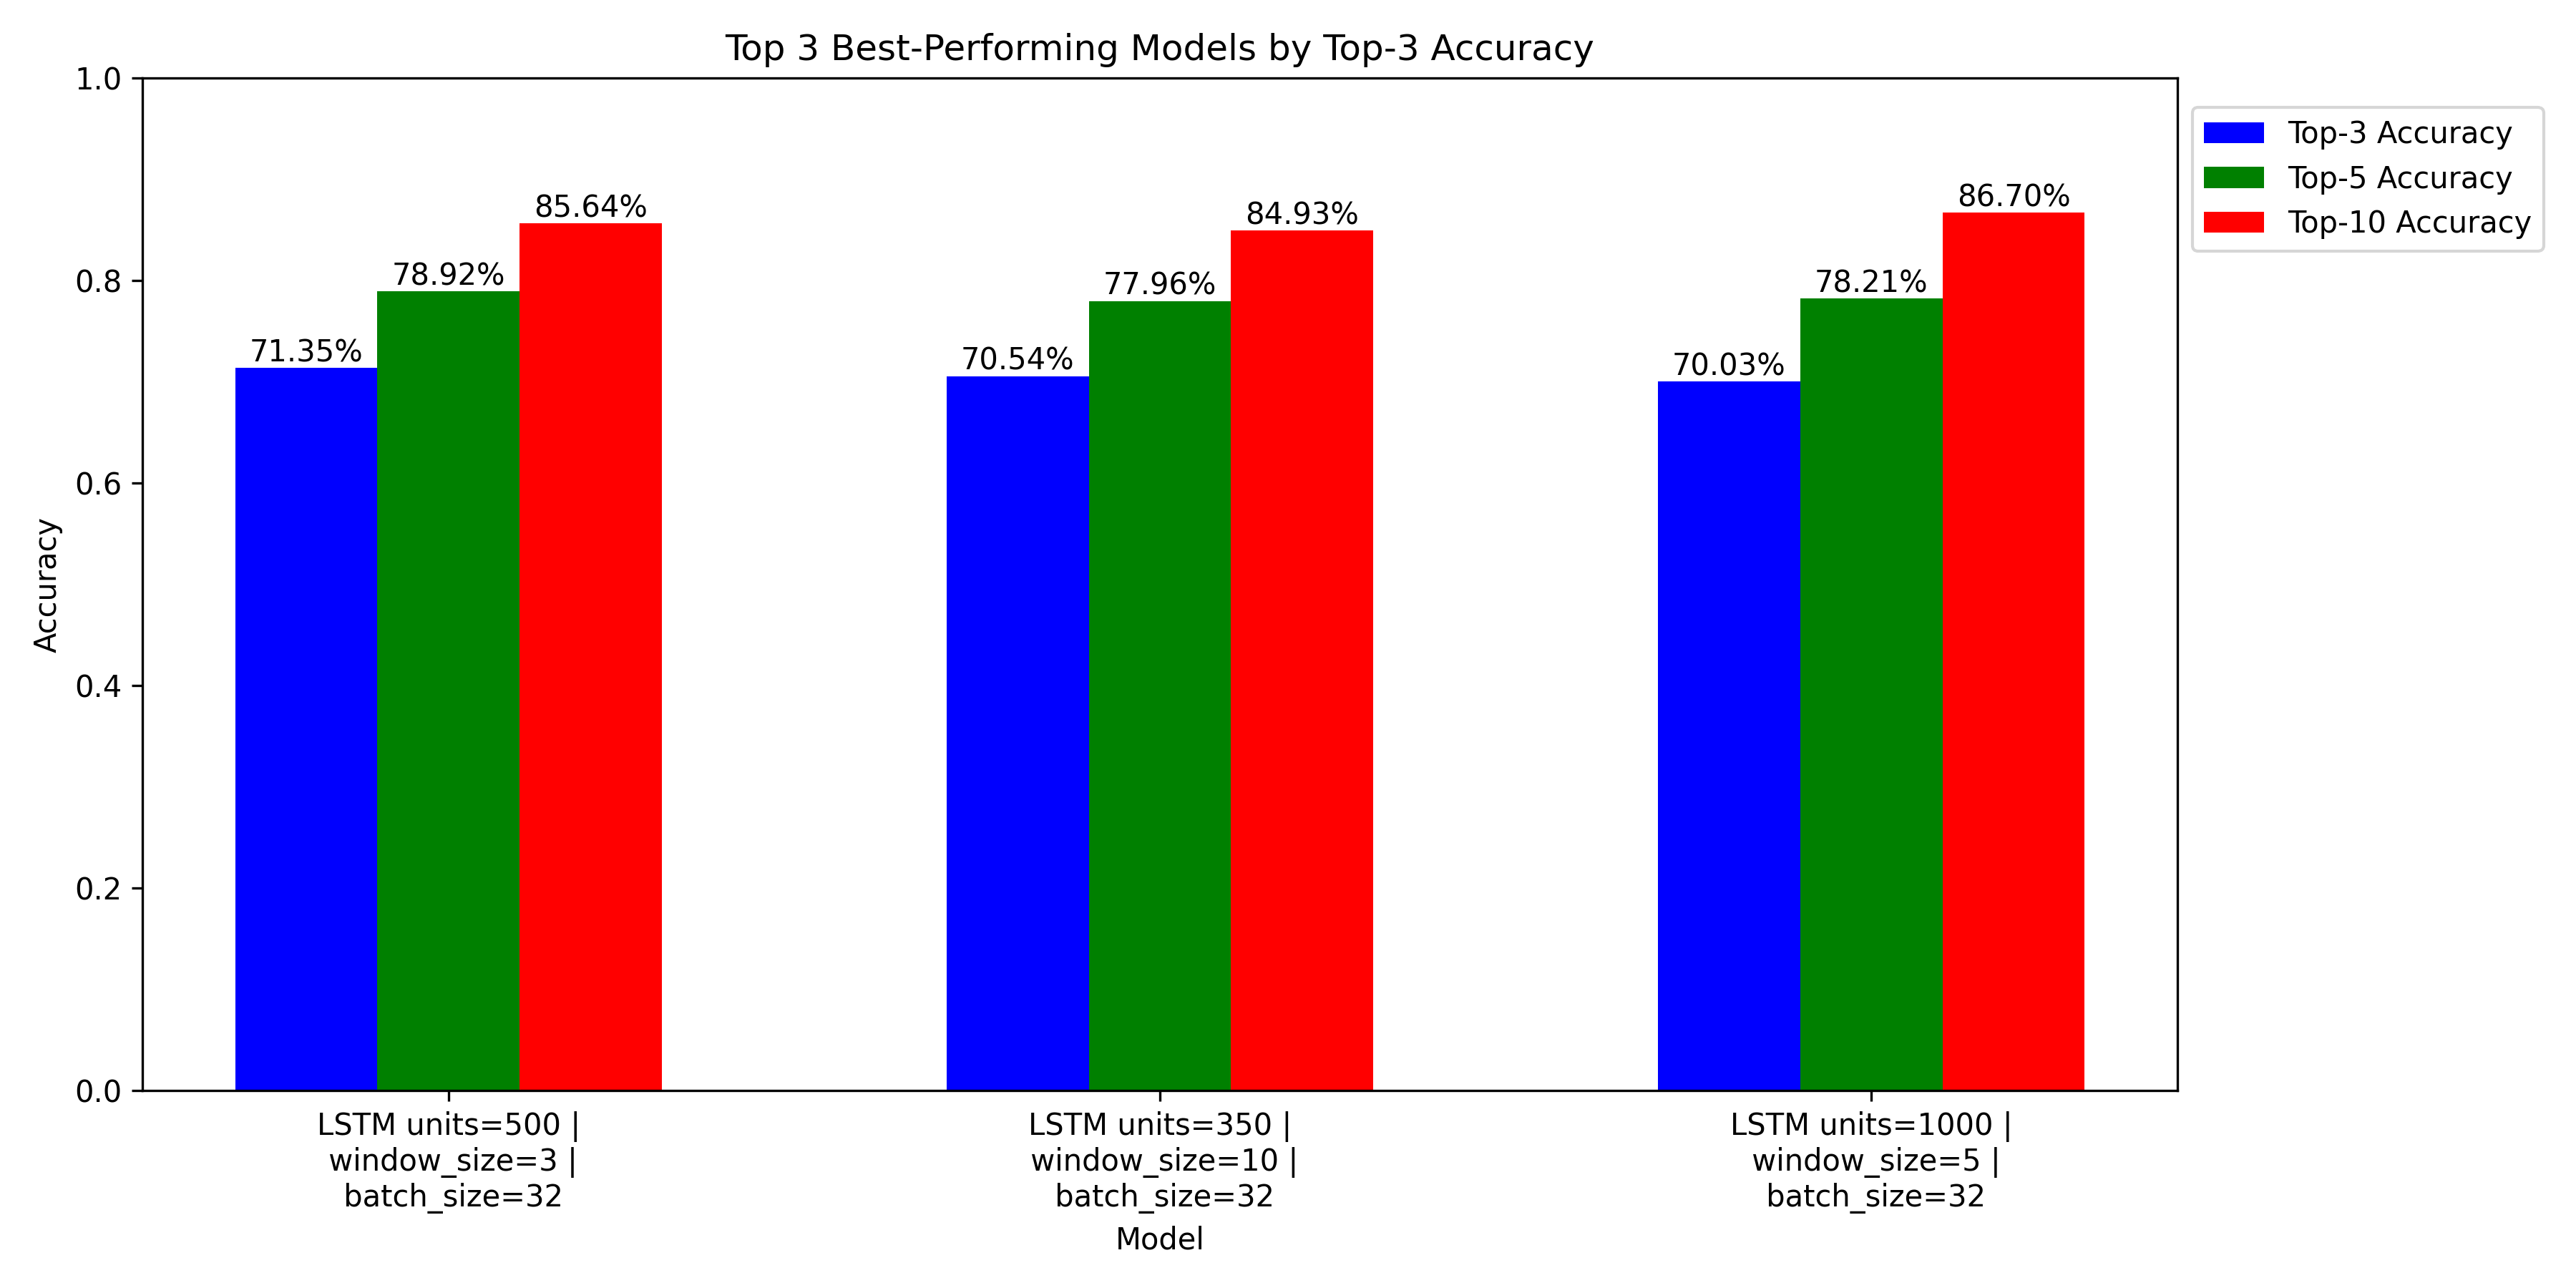
\includegraphics[scale=0.4]{images/top3_best_models.png}
    \caption{Accuracy of the three best performing models of the implementation}
    \label{fig:top3_best_models}
\end{figure}



%\noindent
